\documentclass[12pt]{exam}
\usepackage[utf8]{inputenc}
\usepackage{graphicx} % Allows including images
\usepackage{cool}
\usepackage{tikz}
\usepackage{amsmath}
\usepackage{listings}
\usepackage{pseudocode}
\usepackage[colorlinks = true,
            linkcolor = blue,
            urlcolor  = blue,
            citecolor = blue,
            anchorcolor = blue]{hyperref}
\usepackage{MnSymbol,wasysym}
\usepackage{geometry} % see geometry.pdf on how to lay out the page. There's lots.
\geometry{a4paper} 
\newgeometry{vmargin={20mm}, hmargin={14mm,18mm}}
 
 \lstset{language=Python,keywordstyle={\bfseries \color{blue}}}
 
\begin{document}
\begin{center}
{\large {\bf Stanford CME 241 (Winter 2023) - Assignment 2}}
\end{center}
 
\noindent {\large{\bf Due: 1/23 @ 11:59pm on Gradescope}}

\noindent \textbf{Please solve questions 1, 2 and choose one of questions 3 or 4. }

\noindent Questions 1 and 2 of this homework focus on Markov Processes (MP and MRP) that were taught in class on 1/13 and are covered in Chapter 3 of the book. Questions 3 and 4 cover Markov Decision Processes that will be taught on 1/18 and are covered in Chapter 4 of the book.

\begin{questions}
\question In the classic childhood game of Snakes and Ladders, all players start the the left of square 1 (call this position 0) and roll a 6-sided die to represent the number of squares they can move forward. The goal is to reach square 100 as quickly as possible. Landing on the bottom rung of a ladder allows for an automatic free-pass to climb (e.g. square 4 sends you directly to 14); whereas landing on a snake's head forces one to slide all the way to the tail (e.g. square 34 sends you to 6). Note, this game can be viewed as a Markov Process, where the outcome is only depedent on the current state and not the prior trajectory. In this question, we will ask you to both formally describe the Markov Process that describes this game, followed by coding up a version of the game to get familiar with the RL-book libraries.

\begin{figure}[h]
	\begin{center}
	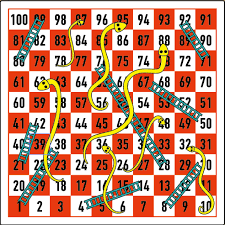
\includegraphics[width=0.4\textwidth]{Figures/2_snakes_and_ladders.png}
	\end{center}
\end{figure}

\begin{enumerate}
	\item[a.] Formalize the state space of the Snakes and Ladders game.
	\item[b.] Write out the structure of the transition probabilities. Feel free to abbreviate all squares that do not have a snake or ladder.
	\item[c.] Code up a \lstinline{transition_map: Transition[S]} data structure to represent the transition probabilities of the Snakes and Ladders Markov Process so you can model the game as an instance of \lstinline{FiniteMarkovProcess}. Use the \lstinline{traces} method to create sampling traces.
	\item[d.] Plot the sample traces and a graph of the distribution of time steps to finish the game.
	\item[e.] For the Snakes and Ladders game, calculate the expected number of rolls to finish the game. Hint: in order to calculate this, extend the Snakes and Ladders FiniteMarkovProcess to an appropriate FiniteMarkovRewardProcess instance. What should be the Rewards model in this MRP so you can use one of the methods in the FiniteMarkovRewardProcess class to determine the expected number of dice rolls to finish the game?
\end{enumerate}
\
\question Consider the problem of a frog jumping across a river with $n=9$ lilypads. The frog at every time step will randomly jump to a position in front of it (e.g. at time step 0, the frog will jump with $\frac{1}{10}$ probability to each of the lilypads or $\frac{1}{10}$ to the other side of the river.)
\begin{figure}
	\begin{center}
		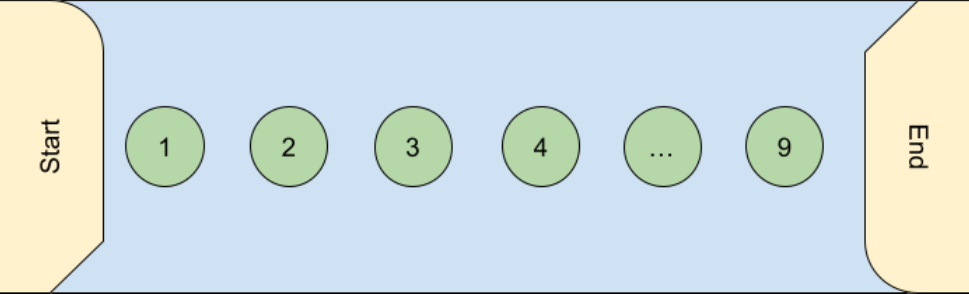
\includegraphics[width=0.5\textwidth]{Figures/2_jumping.png}
	\end{center}
	\caption{A diagram of the frog jumping problem from question 2. }
\end{figure}
\begin{enumerate}
	\item[a.] Formalize the states of the jumping frog problem as well as the structure of the transition probabilites.
	\item[b.] Compute the expected number of steps that it would take for the frog to reach the other side.
	\item[c.] Provide a closed form solution for the expected number of steps / jumps to cross the river. A formal proof is not required. 
\end{enumerate}

 \question Consider an MDP with an infinite set of states $\mathcal{S} = \{1,2,3,\ldots \}$. The start state is $s=1$. Each state $s$ allows a continuous set of actions $a \in [0,1]$. The transition probabilities are given by: $$\mathbb{P}[s+1 \mid s, a] = a, \mathbb{P}[s \mid s, a] = 1 - a \mbox{ for all } s \in \mathcal{S} \mbox{ for all } a \in [0,1]$$
For all states $s \in \mathcal{S}$ and actions $a \in [0,1]$, transitioning from $s$ to $s+1$ results in a reward of $1-a$ and transitioning from $s$ to $s$ results in a reward of $1+a$. The discount factor $\gamma=0.5$.
\begin{enumerate}
	\item[a.] Using the MDP Bellman Optimality Equation, calculate the Optimal Value Function $V^*(s)$ for all $s \in \mathcal{S}$
	\item[b.] Calculate an Optimal Deterministic Policy $\pi^*(s)$ for all $s \in \mathcal{S}$
\end{enumerate}

\question Consider again the problem of a frog jumping across a river with $n-1$ lilypads, labeled $1, \dots, n-1$, with the two riverbanks labeled positions $0$ and $n$. At each time step, the frog who is at lilypad $i$ has two options:
\begin{enumerate}
	\item [(Strategy A)] The frog moves to lilypad $i-1$  with probability $\frac{i}{n}$ and moves to lilypad $i+1$ otherwise.
	\item [(Strategy B)] The frog moves to arbitrary position from $0,\dots,n$ with equal probability.
\end{enumerate}

The frog now starts on a random lilypad. A snake lives on one end of the river (say the snake lives at 0) and will eat the frog if it lands on this side of the river. The frog can escape by landing the other side of the river (i.e. position $n$). What should the frog's strategy be when on each of the lilypads $1, 2, \ldots, n-1$, in order to maximize the probability of escaping the pond (reaching $n$ before reaching $0$)? Although there are more than one ways of solving this problem, we would like to solve it by modeling it as an MDP and identifying the Optimal Policy.\footnote{Sorry for all the frog jumping questions. These games are an easy way to understand Markov Processes, without having to build out too much detail of a financial simulation. Questions will be more related to finance over time.}

\begin{enumerate}
	\item[a.] Express with clear mathematical notation the state space, the action space, transition function, and rewards function of an MDP so that the frog-escape problem would be solved by arriving at the Optimal Value Function (and hence, the Optimal Policy) of the MDP.
	\item[b.] Write code to model this MDP as an instance of the \lstinline{FiniteMarkovDecisionProcess} class. We have learnt that there exists an optimal deterministic policy, and there are $2^{n-1}$ possible deterministic policies for this problem. Write code to create each of these $2^{n-1}$ deterministic policies (as instances of \lstinline{FinitePolicy} class), create a policy-implied Finite MRP for each of these deterministic policies (using the \lstinline{apply_finite_policy} method of \lstinline{FiniteMarkovDecisionProcess} class), and evaluate the Value Function for each of those implied Finite MRPs (using the \lstinline{get_value_function_vec} method of \lstinline{FiniteMarkovRewardProcess} class). This should gives you the Optimal Value Function and the Optimal Deterministic Policy.
	\item[c.] Plot a graph of the Optimal Escape-Probability and of the associated strategies, as a function of the states of this MDP, for $n=3, n=6$ and $n=9$. By looking at the results on this graph, what pattern do you observe for the optimal policy as you vary $n$ from 3 to 9? 
\end{enumerate}

\end{questions}

\begin{figure}[t]
	\begin{center}
		
\includegraphics[width=0.2\textwidth]{Figures/2_frog.png}
	\end{center}
\end{figure}

\end{document}